\documentclass{article}
\usepackage[top=1in, bottom=1in, left=1in, right=1in]{geometry}
\usepackage{graphicx}
\usepackage{minted}

\newcommand{\figref}[1]{Figure~\ref{#1}}
\newcommand{\secref}[1]{Section~\ref{#1}}
\newcommand{\tblref}[1]{Table~\ref{#1}}

\author{Derek Monner}
\title{XLBP Tutorial}
\date{\today}

%\newcommand{\java}{\mintinline{java}}

\begin{document}
\maketitle

\section{Intro}

This document shows you how to build LSTM-like neural networks in Java with XLBP, and train them with the
LSTM-g algorithm. It first covers building networks using convenient pre-built modules. Then we talk about
training and evaluating a network on a data set using cross-validation. Finally, we delve into the
more advanced topics of developing your own training regime and developing your own network
architectures out of more basic components.


\section{Building a Network}

This document shows some example code for building simple LSTM network architectures to be trained 
with LSTM-g. The main class we'll be dealing with is the \mint{java}|Network| class, which holds all information
about the neural network you're building. One adds \mint{java}|Layer|s (or, more often, \mint{java}|Compound|s) to the \mint{java}|Network|
in the order they will be activated during training. The difference between a \mint{java}|Layer| and a \mint{java}|Compound|
rests with the fact that every vector of activation values to be stored, anywhere in the \mint{java}|Network|,
corresponds to an individual \mint{java}|Layer| object; a \mint{java}|Compound|, on the other hand, is generally a collection
of \mint{java}|Layers| wired up in a specific way to create, say, LSTM memory cells with gates. We'll be dealing
exclusively with \mint{java}|Compound|s to start.

\subsection{The Easy Way: Compounds}

First we'll look at code for building the canonical LSTM architecture, where the single hidden layer
of memory cells has input gates, output gates, forget gates, and peephole connections.

\begin{minted}[fontsize=\small]{java}
final String mctype = "IFOP";
final int insize = 5;
final int hidsize = 20;
final int outsize = 2;

final InputCompound in = new InputCompound("Input", insize);
final MemoryCellCompound mc = new MemoryCellCompound("Hidden", hidsize, mctype);
final XEntropyTargetCompound out = new XEntropyTargetCompound("Output", outsize);
out.addUpstreamWeights(mc);
mc.addUpstreamWeights(in);

final Network net = new Network("Canonical LSTM");
net.setWeightUpdaterType(WeightUpdaterType.basic(0.1F));
net.setWeightInitializer(new UniformWeightInitializer(1.0F, -0.1F, 0.1F));
net.add(in);
net.add(mc);
net.add(out);
net.optimize();
net.build();
\end{minted}

The above code starts out simple. We define a few constants, and then we get busy creating \mint{java}|Compound|s
to populate our \mint{java}|Network|. Each \mint{java}|Compound| has an integer size parameter that specifies how many units
go in the associated \mint{java}|Layer|s that make up the \mint{java}|Compound|. So here, we have 5 input units, 20 memory
cells (each with its own set of gates), and 2 output units. The \mint{java}|XEntropyTargetCompound| specifies
that we plan to train the \mint{java}|Network| with a back-propagated cross-entropy error measure.

The \mint{java}|mctype| variable warrants some explanation---it provides a shorthand for specifying what
components we want our \mint{java}|MemoryCellCompound| to contain. If  \mint{java}|mctype| is the empty string, you will get
only memory cells with no gates. Otherwise, you can add the following letters to this string, in any
order, to add the associated components:

\begin{minted}[fontsize=\small]{java}
/*
I = [I]nput gates
F = [F]orget gates
O = [O]utput gates
P = [P]eephole connections
G = Lateral connections from all extant gate units to the memory cell, [G]ated by the input gates
U = Lateral connections from all extant gate units to the memory cell, [U]ngated
*/
\end{minted}
There are also a couple other switches that are used less often and do stranger things:
\begin{minted}[fontsize=\small]{java}
/*
N = Specifies [N]o memory component -- the Compound will not remember values across time steps
T = [T]runcate errors at gates -- turning this on forces the network to ignore error signals
    originating at gate units; this is the behavior of the original LSTM training algorithm, but the
    default LSTM-g training algorithm used here makes use of these errors.
*/
\end{minted}
    
So, to summarize, if you want the original LSTM architecture (input and output gates only, trained
with the original LSTM algorithm), you'd set  \mint{java}|mctype = "IOT"|. If you want all three gate types but don't care about peephole 
connections (and they don't seem to make a lot of difference for many applications), you might use 
 \mint{java}|"IFO"|. And if you want to add ungated lateral connections, as used to great effect in our 2012 paper, you 
want  \mint{java}|"IFOU"|.

There are a few other built-in variations in \mint{java}|MemoryCellCompound| that one can take advantage of. Changing the activation functions used throughout the \mint{java}|Layer|s comprising a \mint{java}|MemoryCellCompound| is as easy as naming the function in the constructor---just add a fourth parameter with the function type, one of ``logistic'' (the default), ``tanh'', or ``linear'':

\begin{minted}[fontsize=\small]{java}
// creates a MemoryCellCompound where the cells and gates
// all use the hyperbolic tangent activation function
final MemoryCellCompound mc = new MemoryCellCompound("Hidden", hidsize, mctype, "tanh");
\end{minted}

There are even more constructors for \mint{java}|MemoryCellCompound| that give you even greater flexibility with regard to the activations functions of each set of gates, whether each unit has biases, etc.

Our example code above specifies a memory cell hidden layer with input, forget, and output gates, as
well as peephole connections. With all the components created, we specify which \mint{java}|Compound|s connect
to each other, and how. The call:
\begin{minted}[fontsize=\small]{java}
out.addUpstreamWeights(mc);
\end{minted}
creates a weight matrix from the memory cell outputs projecting to the output units, and
automatically fills it with small random weight values. The next similarly creates weights between the inputs and the memory cells:
\begin{minted}[fontsize=\small]{java}
mc.addUpstreamWeights(in);
\end{minted}
In fact, this call creates 4 new weight matrices in this
case. Each of these begins at the input layer, and they project to the memory cells and all extant gates; so here, our four weight matrices project to the input gates, forget gates,
output gates, and memory cells. This is the canonical way to connect up an LSTM hidden layer. For greater control on the connectivity, you can use methods on \mint{java}|MemoryCellCompound| to pull out, for example, individual gate layers and give them incoming weights individually. For example: \mint{java}|mc.getForgetGates().addUpstreamWeight(someOtherLayer)|.

With the layers and connectivity complete, all we have to do is collect this information in a 
\mint{java}|Network| instance. We create one on the first line and name it; on the subsequent lines we set a few global properties for the entire \mint{java}|Network|. The \mint{java}|WeightUpdaterType| controls the type of weight updates that the \mint{java}|Network| performs. We recommend using the ``basic'' type, which corresponds to online LSTM-g as described in our paper, but there are also experimental variants that perform batch-updating, include momentum terms, or utilize ``resilient'' features that apply the
ideas behind the RProp algorithm to LSTM-g. For the ``basic'' type, you can specify the learning rate here as a float parameter to \mint{java}|WeightUpdaterType.basic()|. The \mint{java}|WeightInitializer| controls how weight matrices are created. The recommended option is the \mint{java}|UniformWeightInitializer|, which takes a probability $p$ as an argument and will create weight matrices with uniform density of $p$; in other words, each possible connection that could be created between a sending unit and a receiving unit will have a probability $p$ of being created. Many applications will want to simply set $p = 1$ for full connectivity between each pair of layers, but in our experience, sometimes a lower $p$ produces faster networks that also perform better! Your \mint{java}|UniformWeightInitializer| can also specify the upper and lower bounds for initial random weights; in the code below, weights are initialized to a value uniformly chosen from the interval $[-0.1, 0.1]$.

\begin{minted}[fontsize=\small]{java}
final Network net = new Network("Canonical LSTM");
net.setWeightUpdaterType(WeightUpdaterType.basic(0.1F));
net.setWeightInitializer(new UniformWeightInitializer(1F, -0.1F, 0.1F));
\end{minted}

Once the \mint{java}|Network| parameters are set, we must add components to it in the order in which those 
components should be activated during a trial---inputs should generally come first, outputs last, and
layers should be placed in the \mint{java}|Network| in the order of the flow of connectivity from input to
output. Finally, for reasons we won't go into, we call  \mint{java}|optimize()| and  \mint{java}|build()| to get the \mint{java}|Network|
ready for training.

If you wanted to build an architecture with two layers of memory cells in series, you could do
something like this:


\begin{minted}[fontsize=\small]{java}
final InputCompound in = new InputCompound("Input", insize);
final MemoryCellCompound mc = new MemoryCellCompound("Hidden", hidsize, mctype);
final MemoryCellCompound mc2 = new MemoryCellCompound("Hidden2", hidsize, mctype);
final XEntropyTargetCompound out = new XEntropyTargetCompound("Output", outsize);

out.addUpstreamWeights(mc2);
mc2.addUpstreamWeights(mc);
mc.addUpstreamWeights(in);

final Network net = new Network("Canonical LSTM");
net.add(in);
net.add(mc);
net.add(mc2);
net.add(out);
\end{minted}

The only difference here is the creation of the additional  \mint{java}|MemoryCellCompound|, and additional call
to connect it serially to its predecessor, and an extra call to add it to the \mint{java}|Network| itself. Similarly, to add an extra bank of direct weighted connections between, say, the input and output layers, one would simply add the following line:

\begin{minted}[fontsize=\small]{java}
out.addUpstreamWeights(in);
\end{minted}

If you want a more complex network than that, the sky's the limit. XLBP can build and train
practically any second-order neural network; all you have to do is wire up the pieces and feed it
the inputs and outputs. In particular, for applications involving multiple different types of inputs
and/or outputs, you can have one Network that consists of several sub-\mint{java}|Networks|, each of which is
activated in response to a different input, or to produce a difference output.

We've already seen \mint{java}|Compound|s for input layers, memory cells, and cross-entropy-driven
outputs. There are \mint{java}|Compound|s for other things too, including a vanilla hidden layer for
a normal feed-forward back-propagation network (\mint{java}|LogisticCompound|, or \mint{java}|TanhCompound| if you prefer a different activation function), and an output driven by sum-of-squares
error (\mint{java}|SumOfSquaresTargetCompound|). If these built-ins aren't enough for you, though,
you'll need to learn how to build \mint{java}|Network|s using \mint{java}|Layers|s, as discussed 
next. If \mint{java}|Compound|s are fine for you for now, feel free to skip the upcoming section.

\subsection{The Hard Way: Layers}

Under the hood, \mint{java}|Compound|s are all just collections of \mint{java}|Layer|s connected up 
in a pre-specified way. A \mint{java}|Layer| in XLBP is anything that can contain a vector of
activation values. So everything in a neural network that you're used to thinking of as a layer
needs its own XLBP \mint{java}|Layer|; on top of that, any intermediate computational step also
needs its own \mint{java}|Layer|. Essentially, any computation performed by your network will need
to be expressed structurally in \mint{java}|Layer|s expressing sums, products, applications of
differentiable functions like the logistic, and of course multiplications by learned weight
matrices. Spelling everything out directly in the architecture allows XLBP to automatically 
calculate the appropriate gradients, or error responsibilities, assigned to each unit; these are
integral in actually training the network to do real work. Despite the seeming complexity of such an
architecture, XLBP keeps things speedy using a combination of caching, aliasing, and intelligent
updating that works behind the scenes to produce performance every bit as good (if not better) than
most special purpose implementations of individual network architectures, yet with a \textit{lot}
more flexibility.

In general, \mint{java}|Layer|s in XLBP connect \textit{directly} to one another, rather than 
connecting with an intervening trainable weight matrix. A direct connection here implies a couple
things. First, the two directly connected \mint{java}|Layer|s need to have the same number of units.
This is because the output value of unit $i$ in the sending \mint{java}|Layer| is going to be wired
directly to the input of unit $i$ in the receiving \mint{java}|Layer|. This kind of direct
\mint{java}|Layer| wiring allows us to chain computations to create the basic components of more
traditional neural networks. Generally, each \mint{java}|Layer| connects to one upstream layer---that is, the layer that provides its input---and one downstream layer---the layer that receives its output. Of course there are exceptions: \mint{java}|InputLayer|s have no upstream connections for obvious 
reasons, and \mint{java}|TargetLayer|s---where outputs are evaluated against target values---have
no downstream connections. Some \mint{java}|Layer|s, like the \mint{java}|SigmaLayer| and the 
\mint{java}|PiLayer|, add or multiply several upstream inputs to produce a single downstream output;
similarly, the \mint{java}|FanOutLayer| allows a single upstream input to be split and sent to 
multiple downstream destinations simultaneously.

For example, let's think about a hidden layer in a typical feed-forward network that receives a weighted input from another layer as well as a bias for each unit, and
applies the logistic function to the sum of these to produce an output. Such a layer is encapsulated
in XLBP's \mint{java}|LogisticCompound|, and the underlying \mint{java}|Layer| structure is shown in
\figref{fig-hidden}. Starting on the bottom left of the figure, we see a 
\mint{java}|WeightSenderLayer| that holds the activations of the other layer that projects to our
hidden layer. This \mint{java}|WeightSenderLayer| is allowed to be a different size than the hidden
layer, just as in a conventional neural network, because they are separated by a weight-matrix
multiplication that allows the change in dimensionality. The result of that multiplication---the 
as-yet-unbiased weighted input to the hidden layer---is stored in the 
\mint{java}|WeightReceiverLayer|. Nearly all weighted connections in XLBP need to be bookended by a
\mint{java}|WeightSenderLayer| and a \mint{java}|WeightReceiverLayer|. The only exception is a bias
input such as the one on the bottom right of the figure. An instance of \mint{java}|BiasLayer| acts
as a \mint{java}|WeightReceiverLayer| with a vector of weights that act as if they all project from 
a single always-on bias unit. Thus, the activation on the \mint{java}|BiasLayer| is precisely the
value of the bias weight vector. The \mint{java}|SigmaLayer| adds these bias values to the weighted
input calculated on the left side, storing the biased input values. Finally, these are sent to the
\mint{java}|LogisticLayer|, where the activation stored is the result of passing the upstream values
through the logistic function.

\begin{figure}
\centering
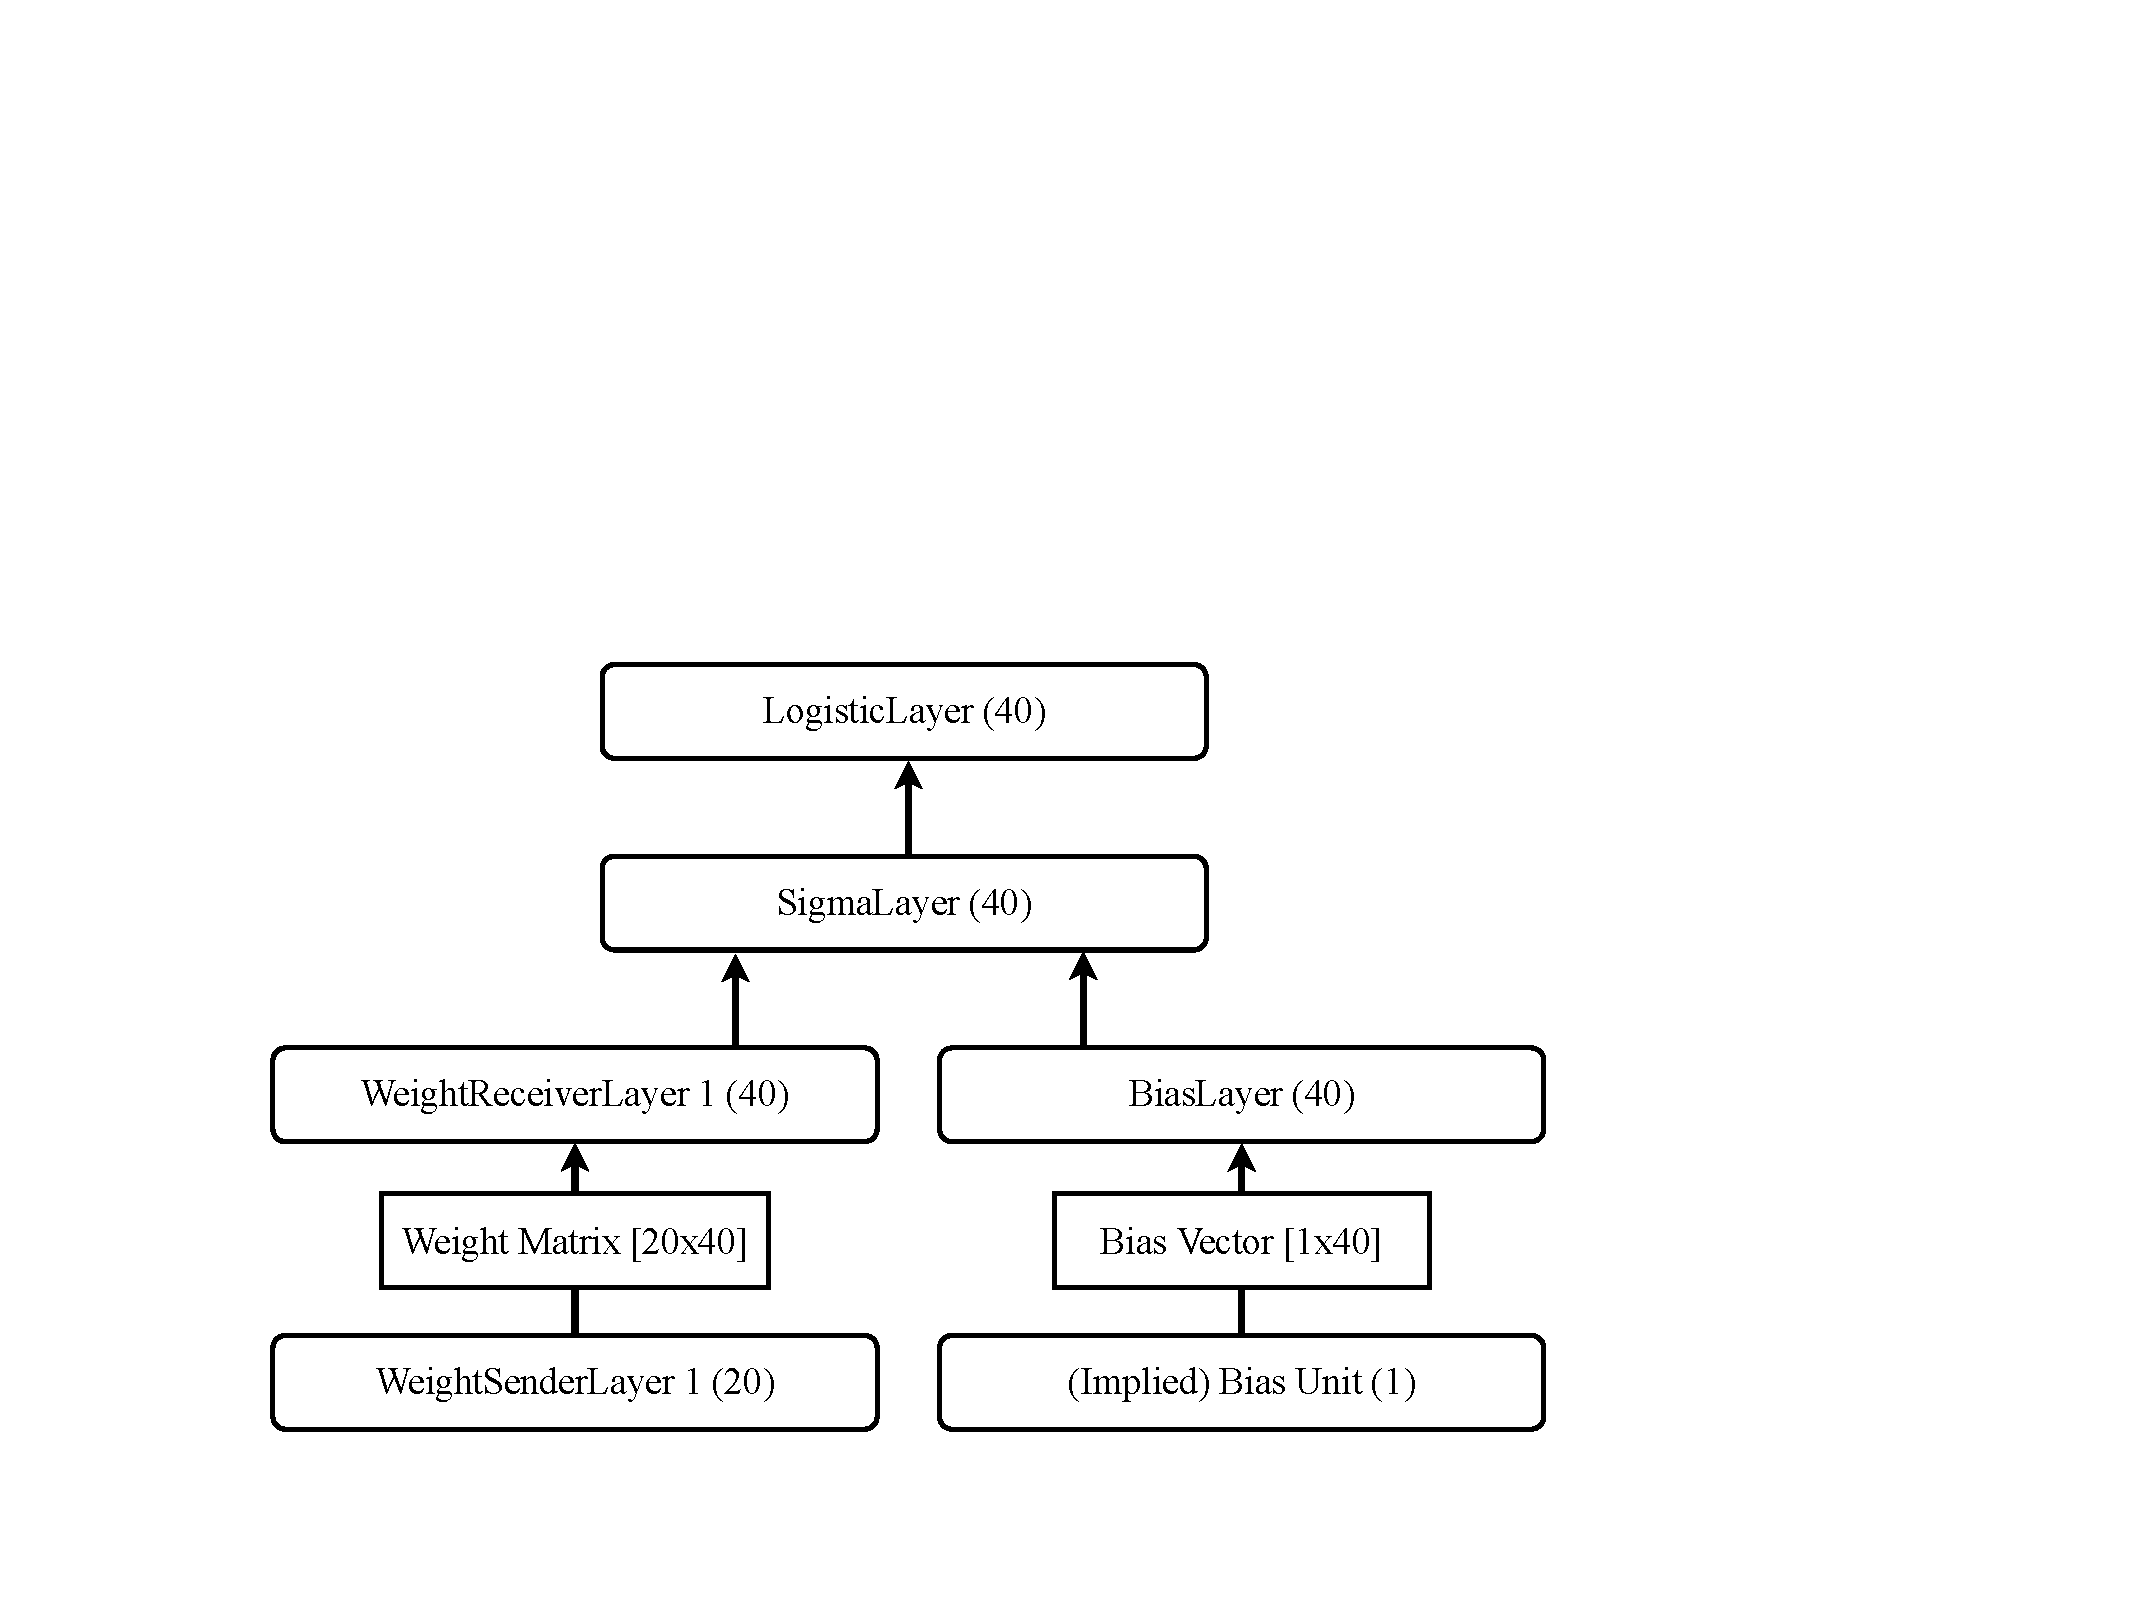
\includegraphics[width=0.6\linewidth]{hidden.pdf}
\caption{A hidden layer of a canonical feed-forward back-propagation network as implemented in XLBP, complete with input weight matrix, biases, and logistic function appliaction.}
\label{fig-hidden}
\end{figure}

Working with \mint{java}|Layer|s is more verbose than using \mint{java}|Compound|s, but otherwise
almost as simple. All you need to do is create the \mint{java}|Layer|s you want, connect them up,
and add them to a \mint{java}|Network|. Here's an example of how you would code up the subnetwork
shown in \figref{fig-hidden}:

\begin{minted}[fontsize=\small]{java}
final int inputSize = 20;
final int hiddenSize = 40;
...

// Create the bookend layers for a weighted connection
final WeightSenderLayer sender = new WeightSenderLayer("Sender", inputSize);
final WeightReceiverLayer receiver = new WeightReceiverLayer("Receiver", hiddenSize);

// Create the weighted connection matrix
final AdjacencyMatrixConnection matrix = new AdjacencyMatrixConnection(receiver, sender);

// Create the bias layer -- automatically makes the bias weight vector
final BiasLayer bias = new BiasLayer("Bias", hiddenSize);

// Create the input-sum layer and the logistic-application layer
final SigmaLayer sigma = new SigmaLayer("Sigma", hiddenSize);
final LogisticLayer logistic = new LogisticLayer("Logistic", hiddenSize);

...

// Connect everything up
...
logistic.addUpstream(sigma);
sigma.addUpstream(bias);
sigma.addUpstream(receiver);
receiver.setConnection(matrix);
...

// Put them into a Network
Network net = new Network("Net");
...
net.add(sender);
net.add(receiver);
net.add(bias);
net.add(sigma);
net.add(logistic);
...
\end{minted}


\section{Examining a Network}

Since building a \mint{java}|Network| is often a complicated endeavor, even with \mint{java}|Compound|s and especially with \mint{java}|Layer|s, XLBP provides a couple easy ways to print, display, or log a wide range of information about the \mint{java}|Network|s you create. Printing and logging are handled by the class \mint{java}|NetworkStringBuilder|, which, as its name implies, builds printable strings describing a \mint{java}|Network|'s architecture, connectivity, weight values, activations values, and just about anything else you might want to examine before, during, or after training a \mint{java}|Network|. A second option is \mint{java}|NetworkDotBuilder|, which allows easy visualization of \mint{java}|Network| structure in conjunction with the standard UNIX graph-processing tool \texttt{dot}.

\subsection{NetworkStringBuilder}
The class \mint{java}|NetworkStringBuilder| was created to facilitate printing and logging data from a \mint{java}|Network|, but one need not used it directly, because the \mint{java}|Network| class's \mint{java}|toString(String show)| method is a convenience wrapper around most of its functionality. The idea of this method is simple: The \mint{java}|show| parameter is a string of letters, in any order, that specify the information about the \mint{java}|Network| that should be returned in printable form. In that way it is much like the \mint{java}|mctype| parameter to the constructor of \mint{java}|MemoryCellCompound|. Here are the values that you can put in a \mint{java}|show| string:

\begin{minted}[fontsize=\small]{java}
/*
Layer-level switches:
N = [N]ame of each layer and weight matrix
C = Upstream and downstream [C]onnectivity for each layer

Unit-level switches:
S = Current pre-activation [S]tate of each unit
A = Current [A]ctivation of each unit
R = Current error [R]eponsibility of each unit

Weight-level switches:
W = [W]eight values in each matrix
E = Current update [E]ligibilities of each weight
L = [L]earning rate of each weight matrix

Advanced switches:
I = [I]ntermediate layers that exist between the important ones
X = Any e[X]tra information that a layer or weight matrix wants to provide
*/
\end{minted}

A good way to evaluate your newly created \mint{java}|Network| is to print or log the output of
\mint{java}|net.toString("NAWL")|, both right after \mint{java}|Network| creation and after a few rounds of training. This will show you all important layers in the \mint{java}|Network|, as well as the activations of the units---so you can make sure they are all getting activated properly---and the weight matrices---so you can check that all the weights are being updated appropriately. More advanced \mint{java}|Network| builders may want to add the \mint{java}|I|, \mint{java}|X|, and \mint{java}|C| options to get a more detailed view of the \mint{java}|Network|'s structure. The \mint{java}|S|, \mint{java}|R|, and \mint{java}|E| options are mostly for debugging new training methods and should not be needed by most XLBP users.

\subsection{NetworkDotBuilder}

Using \mint{java}|NetworkDotBuilder| is very straightforward. Simply construct an instance and pass in the \mint{java}|Network| you want to visualize, then print that result to a file:

\begin{minted}[fontsize=\small]{java}
outfile.println(new NetworkDotBuilder(myNetwork));
\end{minted}

This produces a file containing a dot-language description of the \mint{java}|Layer|s and \mint{java}|Compound|s comprising your \mint{java}|Network|. You can then use the UNIX command-line utility \texttt{dot} to generate, say, a PDF from this dot-file:

\begin{minted}[fontsize=\small]{bash}
dot -Tpdf my-network.dot -o my-network.pdf
\end{minted}

Viewing this PDF will show you the full \mint{java}|Layer|-level structure of the network, with direct connections shown as dashed lines and weight-matrix connections as solid lines. Additionally, each set of \mint{java}|Layer|s that form a \mint{java}|Compound| will be grouped into a box labeled with the \mint{java}|Compound|'s name.

\section{Training and Evaluating a Network}

\subsection{The Easy Way: Cross-Validation}

Training can be done in a couple of ways. The most foolproof is to use the  \mint{java}|Trainer| to
perform cross-validation of your data set, and this is where we'll begin. We start with the notion
of a  \mint{java}|Trial|, which is a sequence of inputs given to the \mint{java}|Network| and the expected outputs it should
generate in response. A  \mint{java}|Trial| knows which \mint{java}|Network| it will be run on, and consists of a sequence of
 \mint{java}|Step|s. These  \mint{java}|Step|s each specify inputs and outputs that should happen on a given time step
of \mint{java}|Network| activation.


\begin{minted}[fontsize=\small]{java}
// Creates a new Trial and sets the Network it will activate
final Trial trial = new Trial(net);

// Optional: Set whether the Trial should clear the Network before proceeding; defaults to true.
trial.setClear(true);

// Optional: This instructs the Trial to record the Network's actual output values (rather than just
// statistics about their correctness); can be useful for post-hoc analysis. Does not record by
// default.
trial.log();

for(... steps in your trial ...)
{
  // Adds a new Step to your Trial; the Trial automatically keeps track of the steps & order.
  final Step step = trial.nextStep();
  
  // Optional: Set the sub-Network to activate on this step; defaults to Trial's Network set above.
  step.setNetwork(stepNet); 
  
  // Note: You can do either or both of the following on a single Step; if you have more than
  // one simultaneous input or target (on different input/output layers) on the same step, use the
  // variants of these methods that allow you to specify the Layer the input or target applies to.
  step.addInput(inputPattern);
  step.addTarget(targetPattern);
  
  // Optional: Tell the Trial to record the activation of the given Layer after this step; these
  // recordings can be saved and used for post-hoc analysis.
  step.addRecord(layerToRecord);
}
\end{minted}


When a  \mint{java}|Trial| is run, the \mint{java}|Network| may first be cleared, and then each  \mint{java}|TrialStep| is run in sequence.
Each step begins by applying all inputs for that step, then activating the step's \mint{java}|Network|, then (if
we're currently training on the step) applying the targets and updating the weights based on the
\mint{java}|Network|'s error.

For many applications, you will have a finite set of training and testing data. For this, you'll
want to keep your  \mint{java}|Trial|s in a  \mint{java}|TrialSet|. You create one as follows:


\begin{minted}[fontsize=\small]{java}
final Trial[] trials = ...
 
... set up trials ...

final String foldSplit = "";
final String xvalSplit = "9/0/1";
final TrialSet set = new TrialSet(trials, foldSplit, xvalSplit);
final Trainer trainer = new Trainer(set);
\end{minted}

Let's begin by talking about \mint{java}|xvalSplit|. This string has 3 fields, separated by slashes. These fields
specify the number of the number of training folds, validation folds, and testing folds, 
respectively. Their sum is the total number of folds. Here, we have specified 9 training and 1 test
fold, for 10 total folds. This corresponds to standard 10-fold cross validation. The  \mint{java}|TrialSet| will
split the data evenly and randomly into 10 groups called folds, and later the Trainer
will use 9 or these folds to train a \mint{java}|Network| and reserve 1 fold to use as novel testing  \mint{java}|Trial|s. In
fact, the \mint{java}|Trainer| will train 10 separate \mint{java}|Network|s in this case, with each tested on a
different fold; this allows it to report the accuracy of your general Network configuration at
generalizing to the entirety of the data set. The \mint{java}|Trainer| will train your \mint{java}|Network| up
through the number of epochs you specify, and the results of the test folds on the final epoch will
be combined for the final analysis.

To take another example, suppose the \mint{java}|xvalSplit| was \mint{java}|"2/1/1"|. Now we have 4 folds, but the procedure
is different because there is a validation fold. Now we train the \mint{java}|Network| on 2 folds---half the
data---and validate on one fold. Validation is like testing, but it allows us to decide where to
stop training. So instead of reporting results from the test set that occurred after the final epoch of training, we look for the
epoch that gave us the best results on the validation set, and then report the results from that epoch on the test set. This can help prevent over-training of a network.
Note that we do not report results on the validation set; that would be statistical cherry-picking!
Instead, we report the results on the testing fold for the epoch with the best validation set score.
These results are again combined across all four \mint{java}|Network| instances trained with different fold-assignments to
provide a comprehensive view of how your architecture performed.

So far we have ignored the \mint{java}|foldSplit| parameter, which one should generally leave blank. The only
exception to this is if your data set has pre-defined fold boundaries that you'd like to use instead
of the default of randomly generated equal-size folds. In this case, you must organize your  \mint{java}|Trial|s so that
those from the same fold form contiguous blocks in the array. If, for example, your data has 4 pre-
defined folds of sizes 12, 10, 8, and 11 trials, respectively, you would set:

\begin{minted}[fontsize=\small]{java}
foldSplit = "12/10/8/11"
\end{minted}

Note that this will fail if the sum of these numbers is not precisely equal to the number of  \mint{java}|Trial|s,
or if the number of folds specified here does not equal the total number specified by \mint{java}|xvalSplit|.

Once your  \mint{java}|TrialSet| and \mint{java}|Trainer| are created, performing the actual training and analysis
is extremely straightforward:


\begin{minted}[fontsize=\small]{java}
final int epochs = 100; // however many passes you want to make over the data
final TestStat summary = trainer.run(epochs);

final int c = summary.getTrials().getActual();
final int n = summary.getTrials().getPossible();
System.out.println("You got " + c + " trials correct out of " + n + "!");
\end{minted}

Assuming 10-fold cross-validation as in our example above, the second line here will train ten
independent \mint{java}|Network| instances on the 9/1 train-test split and combine the results into a coherent
summary. Be careful---this method can take a while to return if your data set is large and/or if
your \mint{java}|Network| is large and/or if your number of epochs is large. One further caveat when using the 
\mint{java}|Trainer| is that the independent \mint{java}|Network| training sessions are run serially, and the
\mint{java}|Network| is rebuilt (via \mint{java}|net.rebuild()|) before each, meaning that it gets a new set of random
weights. If you need to seed specific weights into your \mint{java}|Network|, you might want to forego 
\mint{java}|trainer.run()| in favor of \mint{java}|trainer.runFold(i)|, or look into the empty hook methods that this class
provides for you to extend with your own functionality.

The returned \mint{java}|TestStat| has all kinds of useful information besides what is displayed in this 
simple example; just have a look at it's methods to find what you need. If you want access to more
granular data about individual  \mint{java}|Trial|s, you can get it via:

\begin{minted}[fontsize=\small]{java}
final TrialStat[] evals = trainer.getEvaluations();
\end{minted}

The result is an array of \mint{java}|TrialStat| objects that each describe how the \mint{java}|Network| handled one of the test-set \mint{java}|Trials|, on the fold where that \mint{java}|Trial| was in the test fold. Each  \mint{java}|TrialStat| holds a reference to the \mint{java}|Trial| that it holds statistics about. If you called \mint{java}|log()|
or \mint{java}|addRecordLayer()| on your \mint{java}|Trial| or  \mint{java}|Step|s, the \mint{java}|TrialStat| will contain copies of the \mint{java}|Network|'s
output values and/or the activations of recorded layers; these recordings can be useful for post-hoc
analysis but are not enabled by default because of the additional memory/time required to generate
and maintain them.


\subsection{The Hard Way: DIY Training Regime}

Cross validation is generally the way to go for fixed-size data sets, but what if you're generating
training and test data on the fly? What if your data set is so large it can't fit in memory? You
could actually define a subclass of \mint{java}|TrialStream| for these situations, and still make use of the
\mint{java}|Trainer|. However, you might find it easier to write your own training/testing code. This 
section will show you the basic outline of a training regime without the aid of a trainer.

\begin{minted}[fontsize=\small]{java}
final float[][][] input = new float[trials][steps][insize];
final float[][][] target = new float[trials][steps][outsize];

... fill in input and target arrays ...

// for each epoch of training
for(int e = 0; e < epochs; e++)
{
  // for each trial in the data set
  for(int t = 0; t < trials; t++)
  {
    // Reset the network's activation levels prior to starting the trial; this is optional.
    // You should make sure NOT to clear() before each step in the same trial--only between trials.
    net.clear();
    
    // for each sequential step in the trial
    for(int s = 0; s < steps; s++)
    {
      // Note: You can do input alone, output alone, or both together on a single step
    
      // INPUT
      // Put the input pattern on the InputCompound; activate the Network and update each unit's
      // weight-update "eligibility" in preparation for training.
      in.setInput(input[t][s]);
      net.activateTrain();
      net.updateEligibilities();
      
      // OUTPUT
      // Tell the output units what target pattern they should expect to see; then have the Network
      // work backwards from the outputs, calculating each unit's error responsibility; then, update
      // the weights on all connections.
      out.setTarget(target[t][s]);
      net.updateResponsibilities();
      net.updateWeights();
    }
  }
}
\end{minted}


The above code with comments should be pretty self-explanatory for the general case of training
without a trainer. Once your \mint{java}|Network| is trained, you can run a faster testing pass over your data
set and gather some statistics about your trained \mint{java}|Network|'s performance:

\begin{minted}[fontsize=\small]{java}
// for each trial in the data set
for(int t = 0; t < trials; t++)
{
  // Reset the network's activation levels prior to starting the trial; this is optional.
  // You should make sure NOT to clear() before each step in the same trial--only between trials.
  net.clear();
  
  // for each sequential step in the trial
  for(int s = 0; s < steps; s++)
  {
    // Note: You can do input alone, output alone, or both together on a single step
  
    // INPUT
    // Put the input pattern on the InputCompound; activate the Network, but don't save the data
    // necessary for weight training -- this saves computation time!
    in.setInput(input[t][s]);
    net.activateTest();
    
    // OUTPUT ANALYSIS
    // Determine here whether the Network has produced the correct answer by comparing the target
    // output pattern target[t][s] with the Network's output pattern; you can get the latter via
    // out.getActivations() or net.getTargetLayer().getActivations(). The comparison can be of your
    // own design, or you can use something like dmonner.xlbp.util.BitStat.compare(.)
  }
}
\end{minted}


\end{document}

